%Dave's handout 7.1-7.2 (Functions of Several Variable/Partial Derivatives)

\vspace{-0.25 in}
\begin{framed}
\subsection*{Objectives}
\begin{itemize}
    \item Be able to determine and interpret \textbf{partial derivatives} of a function of two variables in different applications.
    
\end{itemize}

%%%Reading Assignment%%%
\subsection*{Suggested Reading:}
\begin{itemize}
\item \cite{Calaway}\footnotemark[1]
   \begin{itemize}
        \item \emph{Section 4.1 Functions of Two Variables}
        \begin{itemize}
            \item Functions of Two Variables
            \item Formulas and Tables
            \item Graphs
            \item Functions of Two Real-Life Variables
        \end{itemize}
    \end{itemize}
\end{itemize}
%\subsection*{Supplemental Materials:}
%%%Key Terms%%%
\subsection*{Key Terms and Concepts:} 

\begin{multicols}{2}
\begin{itemize}
    \item Rate of change of a function of more than one variable
    
\end{itemize}
\end{multicols}
\end{framed}
\footnotetext[1]{Available free to download from \url{http://www.opentextbookstore.com/details.php?id=14} .}


\newpage
%%%%%%%%%%START LESSON CONTENT%%%%%%%%%%%%%
%\noindent\makebox[\linewidth]{\rule{\textwidth}{0.8pt}}
\Opensolutionfile{ans}[ans26]
\Opensolutionfile{ansL}[ansL26]
%%%%%%%%%%%%%%%%Dave's handout 7.1-7.2 (Functions of Several Variable/Partial Derivatives)
%%%%%%%%%%%%%%%%%%%%%%%%%%%%%Applied Calculus, Calaway, 4.1 Functions of Two Variables
\noindent To this point, all of the functions we have analyzed have been functions of one variable such as a population function for a community which we have denoted by $P(t)$. Clearly, there are many “factors” that come into play that have an effect on a community’s population over time; for example, there are economic factors and social factors that may play a role in whether the population is predicted to be increasing or decreasing over time. Real life is rarely as simple as one input – one output. Many relationships depend on lots of variables. Here are some more examples: \\
\begin{itemize}[leftmargin=*]
    \item If we consider the value of an account which compounds interest continuously, we have seen that the value depends on the initial amount we invest, $P$, the interest rate, $r$, and time, $t$, over which the initial investment grows.  So technically, the model $A(t)=Pe^{rt}$ is an oversimplification since the only independent variable is time.  It may be more informative in terms of analysis to represent the amount in the account as a \textbf{function of more than one variable:}  $A(P,r,t)=Pe^{rt}$.  Note that to evaluate this function, we need inputs for each of the \textbf{independent variables} $P$,$r$, and $t$.
    \item The air resistance on a wing in a wind tunnel depends on the shape of the wing, the speed of the wind, the wing’s orientation (pitch, yaw, and roll), plus a myriad of other things that I can’t begin to describe.
    \item The amount of your television cable bill depends on which basic rate structure you have chosen and how many pay-per-view movies you ordered.
\end{itemize}
\noindent Since the real world is so complicated, we want to extend our calculus ideas to functions of several variables. If $X_1, X_2, X_3,..., X_n$ are real numbers, then $\left(X_1, X_2, X_3,..., X_n\right)$ is called an $n-$tuple. This is an extension of ordered pairs and triples. A function of n variables is a function whose domain is some set of $n-$tuples and whose range is some set of real numbers. \\
\noindent For much of what we do here, everything would work the same if we were working with 2, 3, or 47 variables. Because we’re trying to keep things a little bit simple, we’ll concentrate on functions of two variables.

\begin{tcolorbox}[title = {A Function of Two Variables}]

\noindent A function of two variables is a function – that is, to each input is associated exactly one output.\\

The inputs are ordered pairs, $(x, y)$. The outputs are real numbers. The domain of a function is the set of all possible inputs (ordered pairs); the range is the set of all possible outputs (real numbers).\\

The function can be written $z = f(x,y)$.\\

Functions of two variables can be described numerically (a table), graphically, algebraically (a formula), or in English.\\

We will often now call the familiar $y = f(x)$ a function of one variable.

\end{tcolorbox}

\begin{example}
The cost $C(d,m)$ in dollars for renting a car for $d$ days and driving it $m$ miles is given by the formula $C(d,m)=40d+0.15m$
\renewcommand{\labelenumi}{\textbf{(\alph{enumi})}}
\begin{enumerate}[leftmargin=*]
    \item What is the cost of renting a car for 3 days and driving it 200 miles? \newpage
    \item What is $C(100,4)$? What is $C(4,100)$?\vspace*{1 in}
    \item Suppose we rent the car for 3 days. Is $C$ an increasing function of miles?\vspace*{1 in}

    \end{enumerate}
    \begin{sol}
    \renewcommand{\labelenumi}{\textbf{(\alph{enumi})}}
    \begin{enumerate}[leftmargin=*]
    \item $C(3,200)=$ \$150.  
    \item $C(100,4) $ represents the cost of renting a car for 100 days and driving it for 4 miles. $C(100,4) $ represents the cost of renting a car for 4 days and driving it for 100 miles. Notice that $C(100,4)$ makes more sense!
    \item If $d$ is fixed to be $d=3$, $C(d,m)$ becomes $C(3,m)=120+0.15m$ which is simply a linear function with a positive slope of 0.15. With the positive slope, this is an increasing function.
    \end{enumerate}
    \end{sol}
    %%solution
    \begin{solL}
    Complete solution here.....
    
    \end{solL}
    
\end{example}
\noindent The graph of a function of two variables is a surface in three-dimensional space. Let's start by looking at the 3–dimensional rectangular coordinate system, how to locate points in three dimensions, and distance between points in three dimensions.\\

\begin{wrapfigure}[10]{r}{0.5\textwidth}

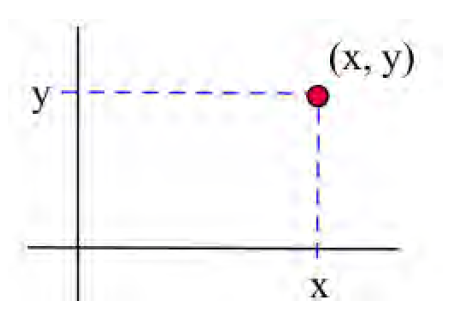
\includegraphics[scale=0.6]{images/twoVariables/2dimGraph.png}
\caption{ }
\label{fig:2dimGraph}
\end{wrapfigure}
\noindent In the 2–dimensional rectangular coordinate system we have two coordinate axes that meet at right angles at the origin, and it takes two numbers, an ordered pair $(x, y)$, to specify the rectangular coordinate location of a point in the plane (2 dimensions). Each ordered pair $(x, y)$ specifies the location of exactly one point, and the location of each point is given by exactly one ordered pair $(x, y)$. The $x$ and $y$ values are the coordinates of the point $(x, y)$.\\

\begin{wrapfigure}[12]{l}{0.5\textwidth}

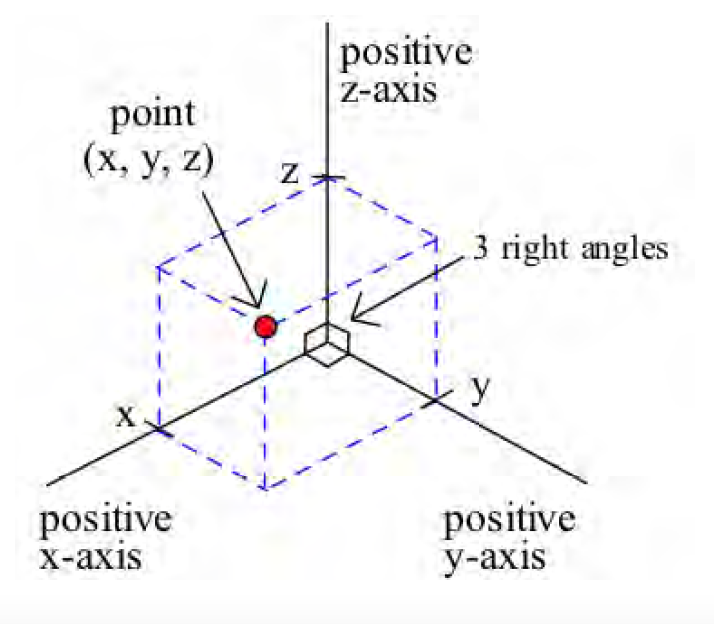
\includegraphics[scale=0.45]{images/twoVariables/3dimGraph.png}
\caption{ }
\label{fig:3dimGraph}
\end{wrapfigure}

\noindent The situation in three dimensions is very similar. In the 3–dimensional rectangular coordinate system we have three coordinate axes that meet at right angles, and three numbers, an ordered triple $(x, y, z)$, are needed to specify the location of a point. Each ordered triple $(x, y, z)$ specifies the location of exactly one point, and the location of each point is given by exactly one ordered triple $(x, y, z)$. The $x$, $y$ and $z$ values are the coordinates of the point $(x, y, z)$. \\
%\hfill \break
%\hfill \break
%\hfill \break
%\hfill \break

\begin{wrapfigure}[7]{r}{0.5\textwidth}

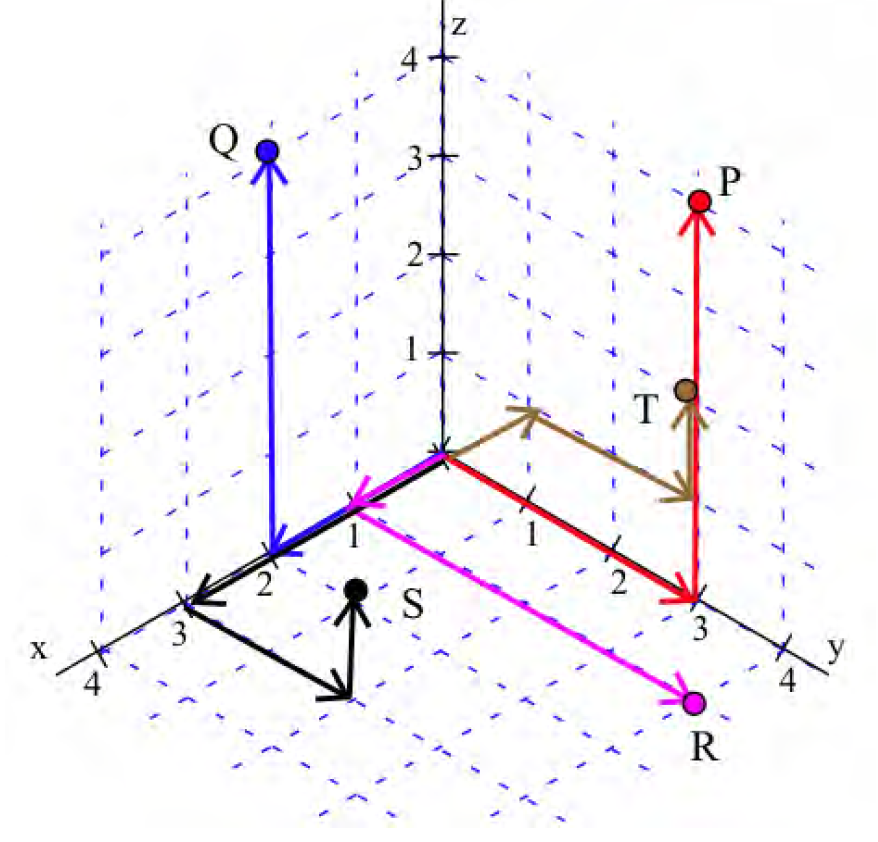
\includegraphics[scale=0.3]{images/twoVariables/3dimEx.png}
\caption{ }
\label{fig:3dimEx}
\end{wrapfigure}

\noindent Figure \ref{fig:3dimEx} is an example of the plot of the locations of the following points on the 3–dimensional rectangular coordinate system:\\
$P=(0,3,4)$\\
$Q=(2,0,4)$\\
$R=(1,4,0)$\\
$S=(3,2,1)$ and $T=(-1,2,1)$\\

\noindent Once we can locate points, we can begin to consider the graphs of various collections of points. By the graph of "$z = 2$" we mean the collection of all points $(x, y, z)$ which have the form "$(x, y, 2)$". Since no condition is imposed on the $x$ and $y$ variables, they take all possible values. The graph of $z = 2$ is a plane parallel to the $xy–$plane and 2 units above the $xy–$plane. Similarly, the graph of $y = 3$ is a plane parallel to the $xz–$plane , and $x = 4$ is a plane parallel to the $yz–$plane. (Note: The planes have been drawn as rectangles, but they actually extend infinitely far.)
\begin{figure}[h!]
    \centering
    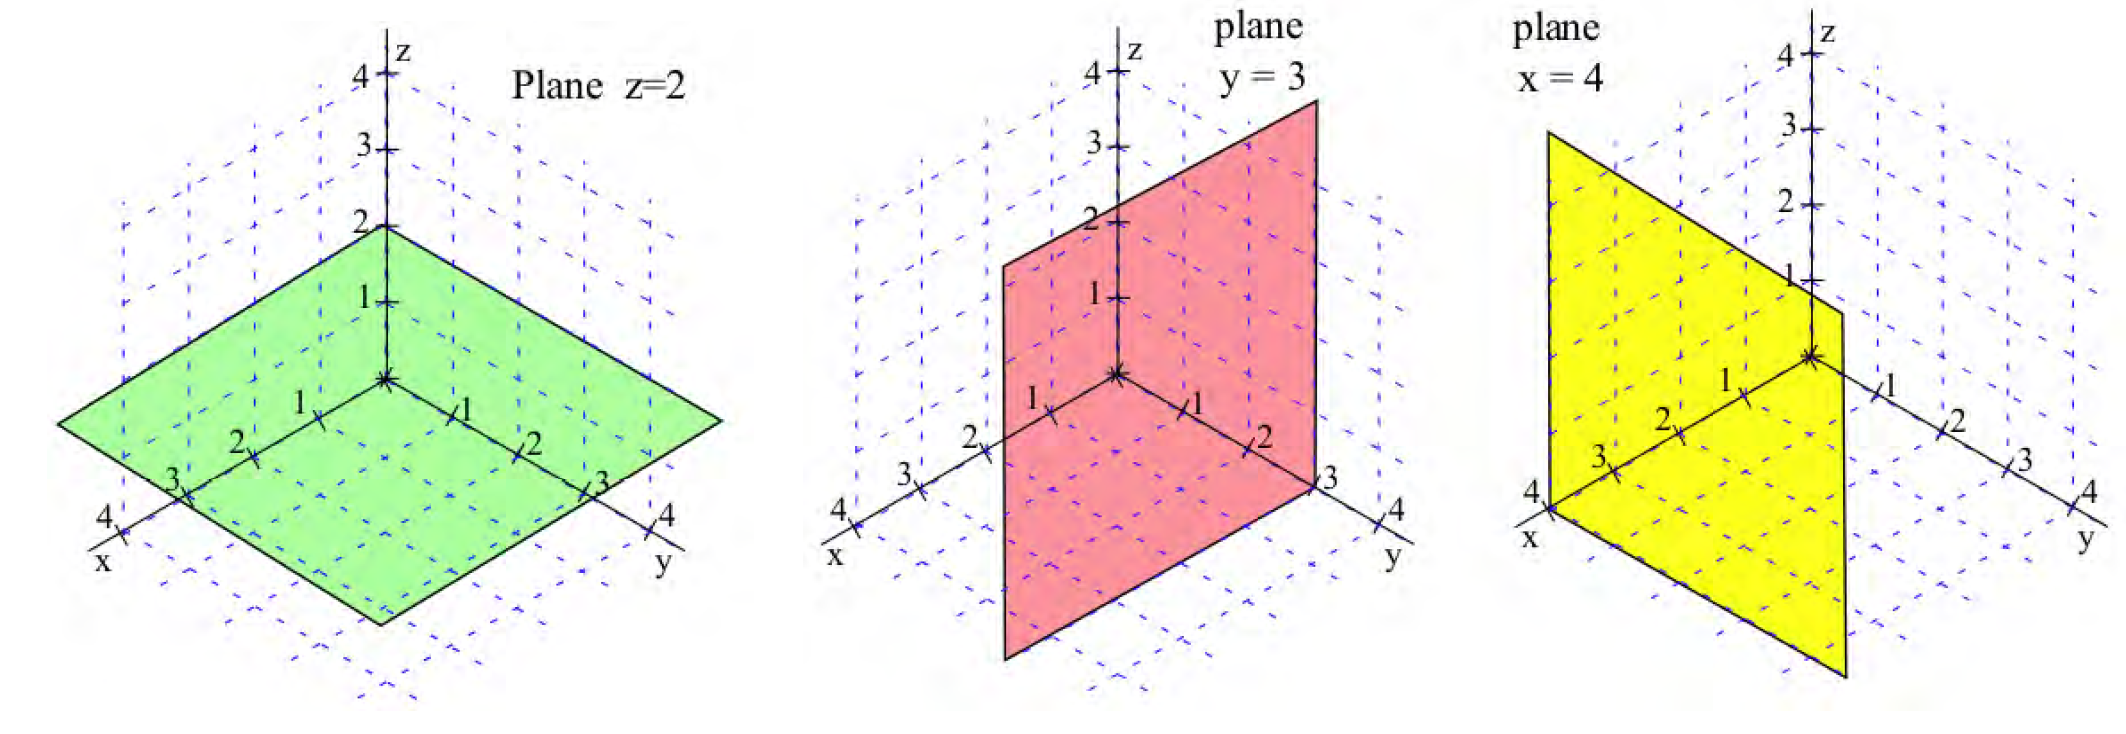
\includegraphics[scale=0.4]{images/twoVariables/planeEx.png}
    \caption{}
    \label{fig:planeEx}
\end{figure}

\noindent Of course, when we move beyond the case of a single independent variable, we lose the luxury of examining a graph of a function in the $x-y$ coordinate system.  As such, the relationships between the \textbf{independent variables} and the value of the function are more difficult to visualize.\\

\noindent Imagine a surface, the graph of a function of two variables. Imagine that the surface is smooth and has some hills and some valleys. Concentrate on one point on your surface. What do we want the derivative to tell us? It ought to tell us how quickly the height of the surface changes as we move. But, which direction do we want to move? This is the reason that derivatives are more complicated for functions of several variables – there are so many directions we could move from any point. As such, the idea of fixing one variable and watching what happens to the function as the other changes is the key to extending the idea of derivatives to more than one variable. This idea is the concept of \textbf{partial derivatives} that will provide us useful information about the relationships between the \textbf{independent variables} and the value of the function.\\

\begin{tcolorbox}[title = {Partial Derivatives}]
\noindent Suppose that $z = f(x, y)$ is a function of two variables.\\

The \textbf{partial derivative of $f$ with respect to} $\bm{x}$ is the derivative of the function $f(x,y)$ where we think of $x$ as the only variable and act as if $y$ is a constant.\\

The \textbf{partial derivative of $f$ with respect to} $\bm{y}$ is the derivative of the function $f(x,y)$ where we think of $y$ as the only variable and act as if $x$ is a constant.\\

The “with respect to $x$” or “with respect to $y$” part is really important – you have to know and tell which variable you are thinking of as THE \textbf{independent variable}.
\end{tcolorbox}

\begin{tcolorbox}[title = {Notation for the Partial Derivative}]
\noindent Suppose that $z = f(x, y)$ is a function of two variables.\\

\noindent The \textbf{partial derivative of} $\bm{y=f(x)}$ \textbf{with respect to} $\bm{x}$ is written as $f_x (x,y)$, or $z_x$ simply $f_x$\\

\noindent The Leibniz notation is $\displaystyle\frac{\partial f}{\partial x}$, or $\displaystyle\frac{\partial z}{\partial x}$\\

We use an adaptation of the $\displaystyle\frac{\partial z}{\partial x}$ notation to mean "find the partial derivative of $f(x,y)$ with respect to $x$:" $\displaystyle\frac{\partial }{\partial x}(f(x,y))=\frac{\partial f}{\partial x}$\\

\end{tcolorbox}
\noindent \textbf{To compute a partial derivative from a formula}:\\

\noindent If $f(x,y)$ is given as a formula, you can find the partial derivative with respect to $x$ algebraically by taking the ordinary derivative thinking of $x$ as the only variable (holding $y$ fixed).\\

\noindent Similarly, everything here works the same way if we are trying to find the partial derivative with respect to $y$--just think of $y$ as your only independent variable and act as if $x$ is constant.

\begin{example}
Certain tests of kidney performance need to have the results adjusted based on the body surface area, $A$, of the patient.  For a person who weighs $W$ pounds and has height $H$ inches, the following function is used to approximate the person’s body surface area: $A(W,H)=0.1091W^{0.425}H^{0.725}$ square feet.   
\renewcommand{\labelenumi}{\textbf{(\alph{enumi})}}
\begin{enumerate}[leftmargin=*]
    \item Determine the approximate body surface area for a 10-year old patient who weighs 100 pounds and is 48 inches tall.   \vspace*{\stretch{1}}  
    \begin{figure}[h!]
        \flushleft
        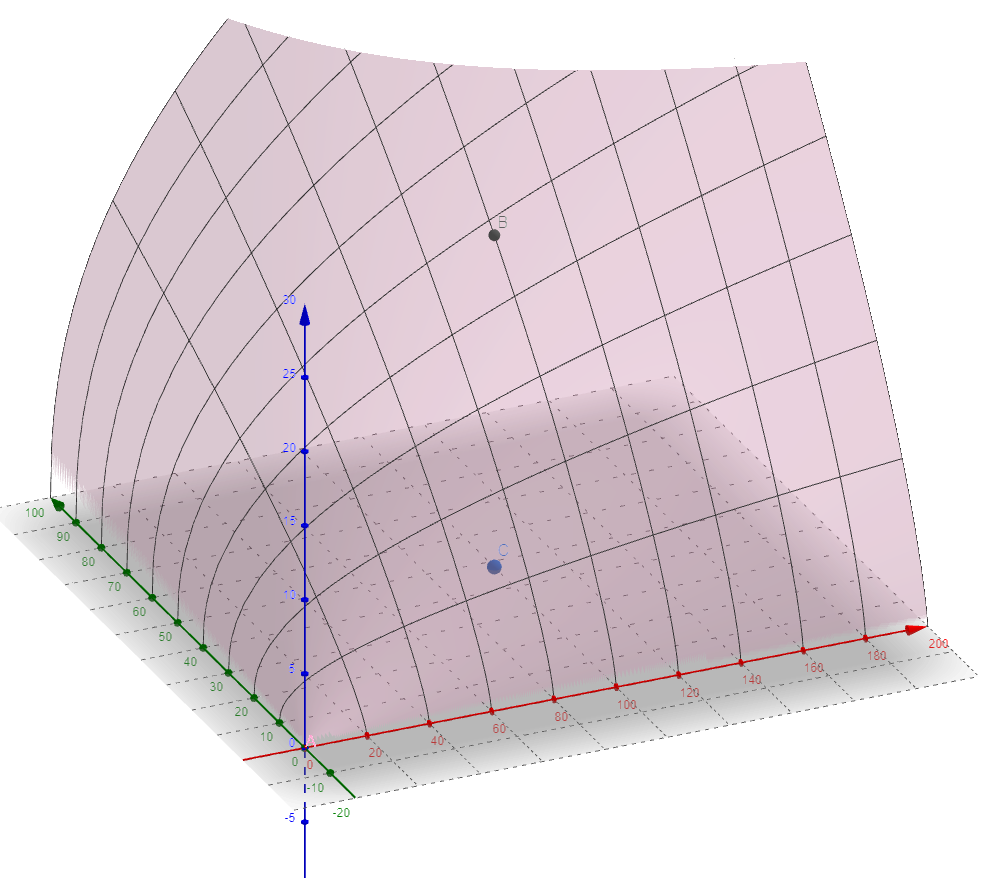
\includegraphics[scale=0.5]{images/twoVariables/ex19_2a.png}
    \end{figure}
    
    \newpage                                    
    \item Determine the \textbf{rate} at which the patient’s body surface area is changing with respect to weight, and the height being held constant. 
    \begin{figure}[h!]
        \flushleft
        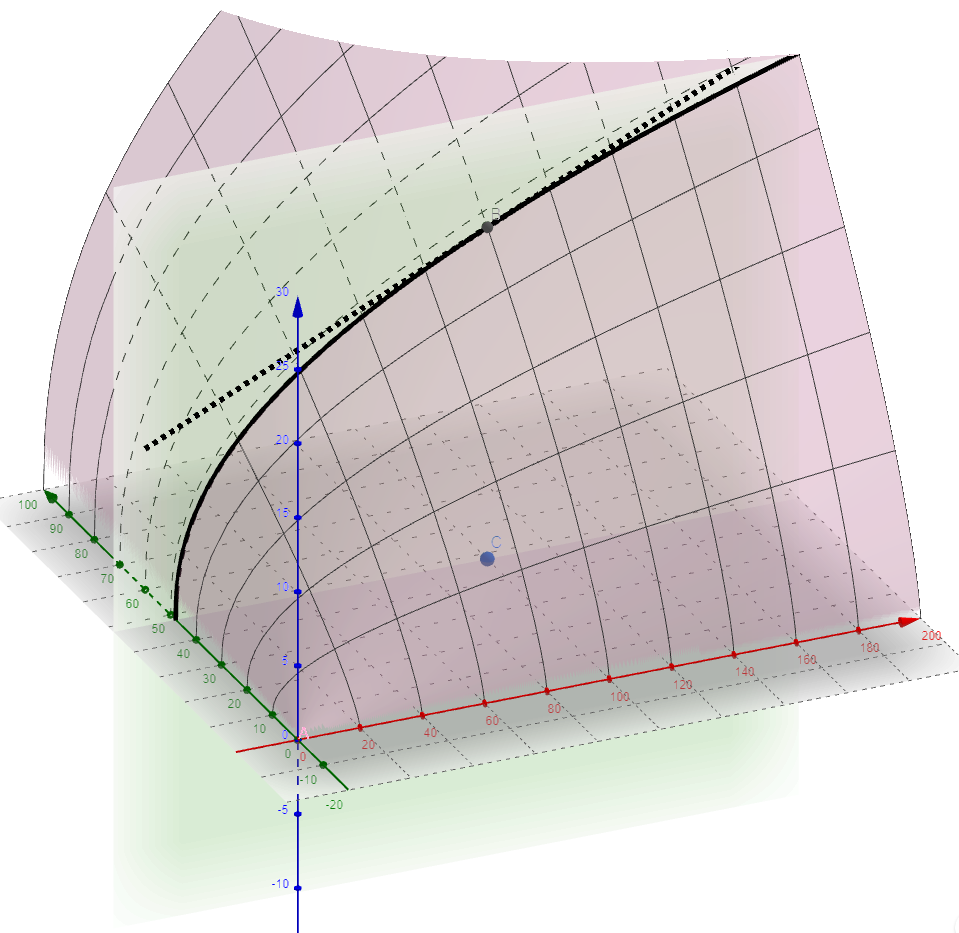
\includegraphics[scale=0.5]{images/twoVariables/ex19_2b.png}
    \end{figure}
    \vspace*{\stretch{1}}  
    \item Determine the \textbf{rate} at which the patient’s body surface area is changing with respect to height, and the weight being held constant.
    \begin{figure}[h!]
        \flushleft
        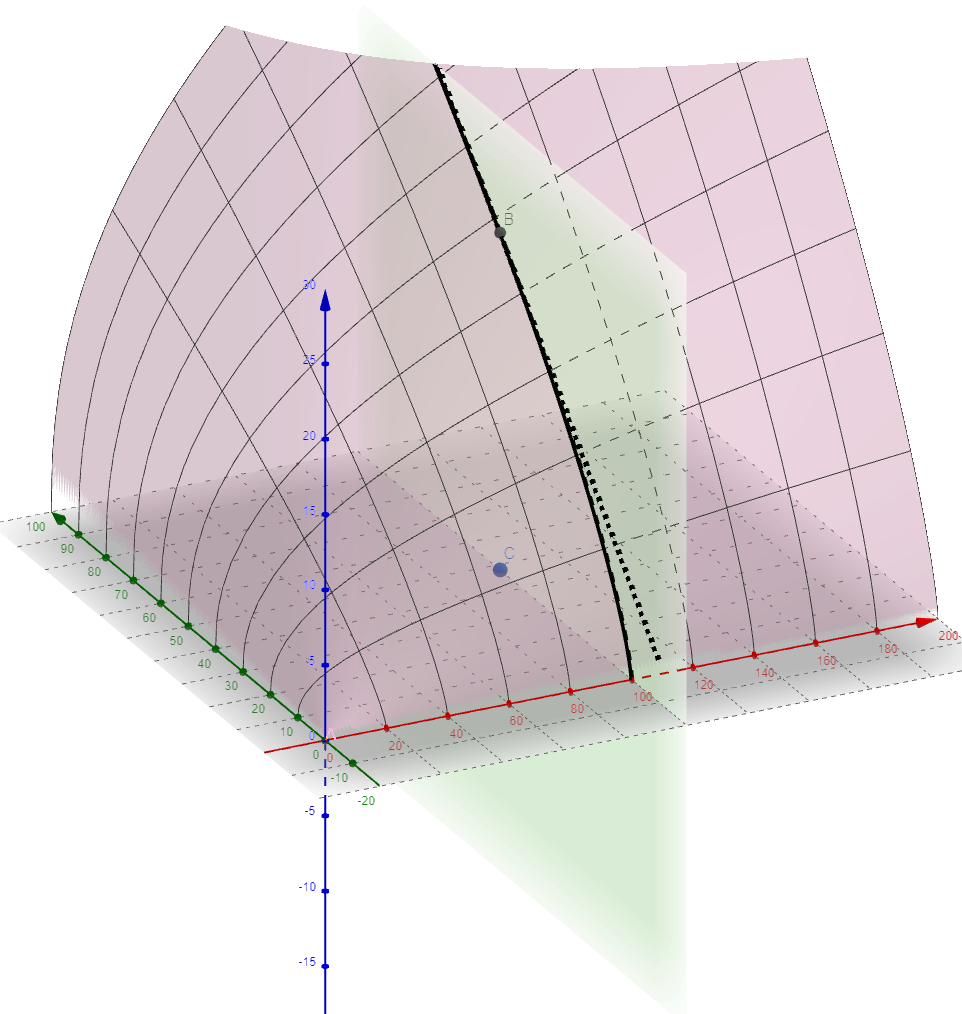
\includegraphics[scale=0.5]{images/twoVariables/ex19_2c.png}
    \end{figure}
    \vspace*{\stretch{1}}  
    \end{enumerate}
    \begin{sol}
    \renewcommand{\labelenumi}{\textbf{(\alph{enumi})}}
    \begin{enumerate}[leftmargin=*]
    \item $A\approx 12.79$ sq.ft.
    \item $\displaystyle \frac{\partial A}{\partial W}=0.046\cdot \frac{H^{0.725}}{W^{0.575}}$ sq.ft.per pound; $\displaystyle \frac{\partial A}{\partial W}\Big|_{W=100,H=48}=0.0543$ sq.ft.per pound; actual change $\approx 0.054187$
    \item $\displaystyle \frac{\partial A}{\partial H}=0.079\cdot \frac{W^{0.425}}{H^{0.275}}$ sq.ft.per inch; $\displaystyle \frac{\partial A}{\partial H}\Big|_{W=100,H=48}=0.193$ sq.ft.per inch; actual change $\approx 0.1883$.
    \end{enumerate}
    \end{sol}
    %%solution
    \begin{solL}
    Complete solution here.....
    
    \end{solL}
    
\end{example}
\newpage
\begin{example}
Biologists model the shape of the bacillus bacteria as a cylinder with 2 spherical caps on each end.  The cylindrical portion has a length denoted by L millimeters and the spherical caps have a radius denoted by r millimeters.   The volume, V, of the shape is given by the function $V(L,r)=\pi r^2 L+\displaystyle\frac{4}{3}\pi r^3$
\renewcommand{\labelenumi}{\textbf{(\alph{enumi})}}
\begin{enumerate}[leftmargin=*]
    \item Determine the rate of change of the volume with respect to a 1 mm. increase in \textbf{length} with the radius being held constant.    \vspace*{\stretch{1}}                                             
    \item Determine the rate of change of the volume with respect to a 1 mm. increase in \textbf{radius} with the length being held constant.  \vspace*{\stretch{1}}  
    \item A certain bacteria is observed to have a length of 4 mm. and a radius of 1 mm.  Which would have a greater impact on the volume, a 1 mm. increase in length or a 1 mm. increase in radius? \vspace*{\stretch{1}}  
    \end{enumerate}
    \begin{sol}
    \renewcommand{\labelenumi}{\textbf{(\alph{enumi})}}
    \begin{enumerate}[leftmargin=*]
    \item  $\displaystyle \frac{\partial V}{\partial L}=\pi r^2$ cubic mm. per mm. length.
    \item $\displaystyle \frac{\partial V}{\partial r}=2\pi rL+4\pi r^2$ cubic mm. per mm. radius.
    \item  $\displaystyle \frac{\partial V}{\partial L}\Big|_{L=4,r=1}=\pi (1)^2\approx 3.14$ cubic mm. per mm. length; $\displaystyle \frac{\partial V}{\partial r}\Big|_{L=4,r=1}=2\pi (1)(4)+4\pi (1)^2\approx 37.7$ cubic mm. per mm. radius; 1 mm. increase in radius has more impact on the volume.
    
    \end{enumerate}
    \end{sol}
    %%solution
    \begin{solL}
    Complete solution here.....
    
    \end{solL}
    
\end{example}
%%%%%%%%%%%%End Examples%%%%%%%%%%%%%%%%%%
%%%%%%%%%%%%%%%End Topic%%%%%%%%%%%%%%%%%%



%%%%%%%%%%%%%%%End Lesson%%%%%%%%%%%%%%%%%%
\Closesolutionfile{ans}
\Closesolutionfile{ansL}

%%%Short Answers to Examples%%%

\newpage
%\vspace*{\fill}
\subsection*{Short Answers to Examples}
%\vspace{-0.25cm}

%\begin{multicols}{2}
\input{ans26}
%\end{multicols}



